\documentclass[orientation=portrait]{beamer}
\beamertemplatenavigationsymbolsempty

\mode<presentation> {\usecolortheme{rose}
}

\usepackage{xcolor}
\usepackage{graphicx}
\usepackage{wrapfig}

\usepackage[all]{xy} % to use xymatrix

\usepackage{mathtools} % to put labels above leftrightarrow

\usepackage{collectbox}

\makeatletter
\newcommand{\mybox}{%
    \collectbox{%
        \setlength{\fboxsep}{1pt}%
        \fbox{\BOXCONTENT}%
    }%
}
\makeatother


\defbeamertemplate{footline}{author and frame number}{%
  \usebeamercolor[fg]{frame number in head/foot}%
  \usebeamerfont{frame number in head/foot}%
  \hspace{1em}\insertshortauthor\hfill%
 page~\insertframenumber ~/ 2 ~
 % \insertframenumber\,/31\,\kern1em\vskip2pt%
% \insertframenumber\,/\,\inserttotalframenumber
}
\setbeamertemplate{footline}[author and frame number]{}

%%%%%%%%%%%%%
%%%%%%%% shortcuts %%%

\newcommand\notch{^{(p)}}
% \newcommand \tilblacktri[1]{{\widetilde{\triangle}_{#1}}}
% \newcommand \blacktri[1]{{\triangle_{#1}}}
% \newcommand \tiltaui[1] {\widetilde{\tau}_{i_{#1}}} 
\newcommand \taui[1] {{\tau_{i_{#1}}}}

% \definecolor{myblue}{cmyk}{1.00,0.56,0.00,0.34}
\definecolor{mygreen}{cmyk}{0.5,0,0.5,0.5}
% \definecolor{myred}{cmyk}{0.00,1.00,0.63,0.00}
% \definecolor{myyellow}{cmyk}{0.00,0.15,1.00,0.00}


\newcommand\puncture{\text{\tiny $P$}}

\newcommand \al {\alpha} \newcommand \be {\beta}
\newcommand\ga{\gamma}  \newcommand\Ga{\Gamma}
\newcommand\ta{\tau } \newcommand\si{\sigma}  \newcommand\Si{\Sigma} 
\newcommand \om {w} \newcommand \oom {$w$}
\newcommand\Cn{\mathcal{C}_n}
\renewcommand\S{S}
\newcommand\Cnn[1]{\mathcal{C}_{#1}}
\newcommand\Z{\mathbb{Z}}
\newcommand\B{\mathcal B} 
\newcommand\AAA {\mathcal A}

\newcommand\TikzPunctureActualSize{0.1}
\newcommand\TikzPointActualSize{0.07}

\newcommand\myemph{\emph}

\newtheorem{conjecture}[theorem]{Conjecture}
\newtheorem{remark}[theorem]{Remark}
\newtheorem{proposition}[theorem]{Proposition}
\newtheorem{furtherdirections}[theorem]{Further Directions}
\newtheorem{result}[theorem]{Result}%{Result 1}
\newtheorem{result2}[theorem]{Result}%{Result 2}
%\newtheorem{proposition}[theorem]{Proposition}
%\newtheorem{goal}[theorem]{Goal}

\newenvironment<>{greenblock}[1]{%
  \begin{actionenv}#2%
      \def\insertblocktitle{#1}%
      \par%
      \mode<presentation>{%
        \setbeamercolor{block title}{fg=black,bg=green!20}
       \setbeamercolor{block body}{fg=black,bg=green!3}
      % \setbeamercolor{itemize item}{fg=orange!20!black}
       %\setbeamertemplate{itemize item}[triangle]
     }%
      \usebeamertemplate{block begin}}
    {\par\usebeamertemplate{block end}\end{actionenv}}


%%%%% shortcuts %%%%%
%%%%%%%%%%%%%%%

%%%%%%% TIKZ %%
%\input{slides_figures}  %%%%
\usepackage{tikz}
\usetikzlibrary{matrix}
\tikzset{->-/.style={decoration={
  markings,
  mark=at position #1 with {\arrow{stealth}}},postaction={decorate}}}
 %%%%%% TIKZ %%%

\usetikzlibrary{decorations.pathreplacing,decorations.markings}

\definecolor{myblue}{cmyk}{1.00,0.56,0.00,0.34}
\definecolor{mygreen}{cmyk}{0.5,0,0.5,0.5}
\definecolor{myred}{cmyk}{0.00,1.00,0.63,0.00}

\tikzset{
  % style to apply some styles to each segment of a path
  on each segment/.style={
    decorate,
    decoration={
      show path construction,
      moveto code={},
      lineto code={
        \path [#1]
        (\tikzinputsegmentfirst) -- (\tikzinputsegmentlast);
      },
      curveto code={
        \path [#1] (\tikzinputsegmentfirst)
        .. controls
        (\tikzinputsegmentsupporta) and (\tikzinputsegmentsupportb)
        ..
        (\tikzinputsegmentlast);
      },
      closepath code={
        \path [#1]
        (\tikzinputsegmentfirst) -- (\tikzinputsegmentlast);
      },
    },
  },
  % style to add an arrow in the middle of a path
  mid arrow/.style={postaction={decorate,decoration={
        markings,
        mark=at position .5 with {\arrow[#1]{stealth}}
      }}},
}
 %%%%%% TIKZ %%%
%%%%%%%%%%%%%%%%%%%%%%%%
%%%%%%%%%%%%%%%%%%%%%%%%%
%%%%%%%%%%%%%%%%%%%%%%%%%%

\begin{document}

\title{Friezes, triangulations, \\ continued fractions, and binary numbers}  
\author[]
%[E. Gunawan\hspace{15em}
%\texttt{umn.edu/home/egunawan}
%Cluster Algebras from Triangulations of %Surfaces]
{{ Emily Gunawan}\\
 {University of Connecticut}\\
 %\texttt{egunawan.github.io} \\
 [6mm]
%(Joint work with Gregg Musiker %(University of Minnesota) 
%and %\\ 
%Hannah Vogel) % (University of Graz)
} 




\newcommand{\zehn}{\hspace{10pt}}
\newcommand{\fuenf}{\hspace{5pt}}
\newcommand{\fuenfm}{\hspace{-5pt}}







 \begin{frame}
 \frametitle{Frieze vectors and unitary friezes}
\begin{columns}
\begin{column}{0.5\textwidth}
      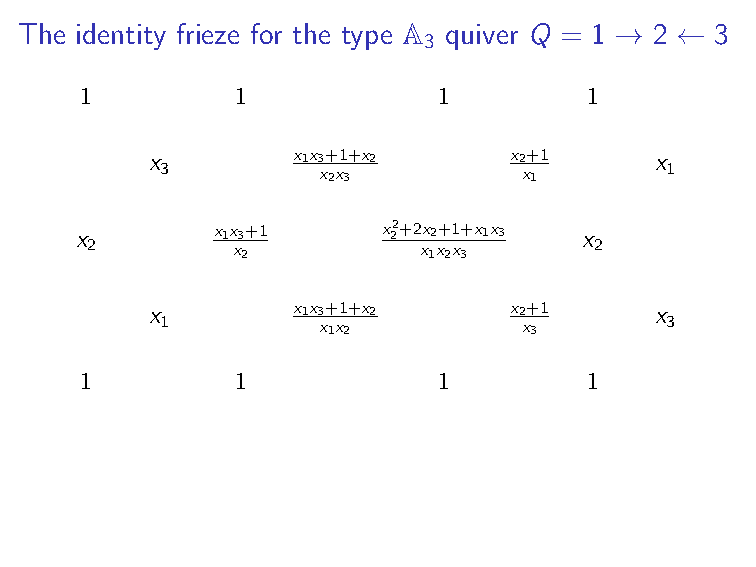
\includegraphics[width=1.2\textwidth]
   {handoutpage1lefttop.pdf} 
   \vskip -1.0cm
   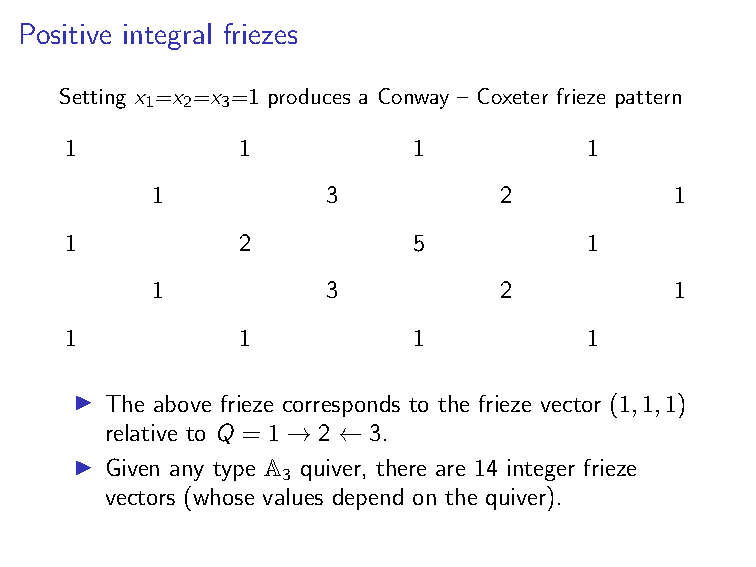
\includegraphics[width=1.2\textwidth]
   {handoutpage1leftbottom.pdf}
\end{column}
\begin{column}{0.56\textwidth}  %%<--- here
    \begin{center}
\vskip -2.9cm
%\begin{figure}
     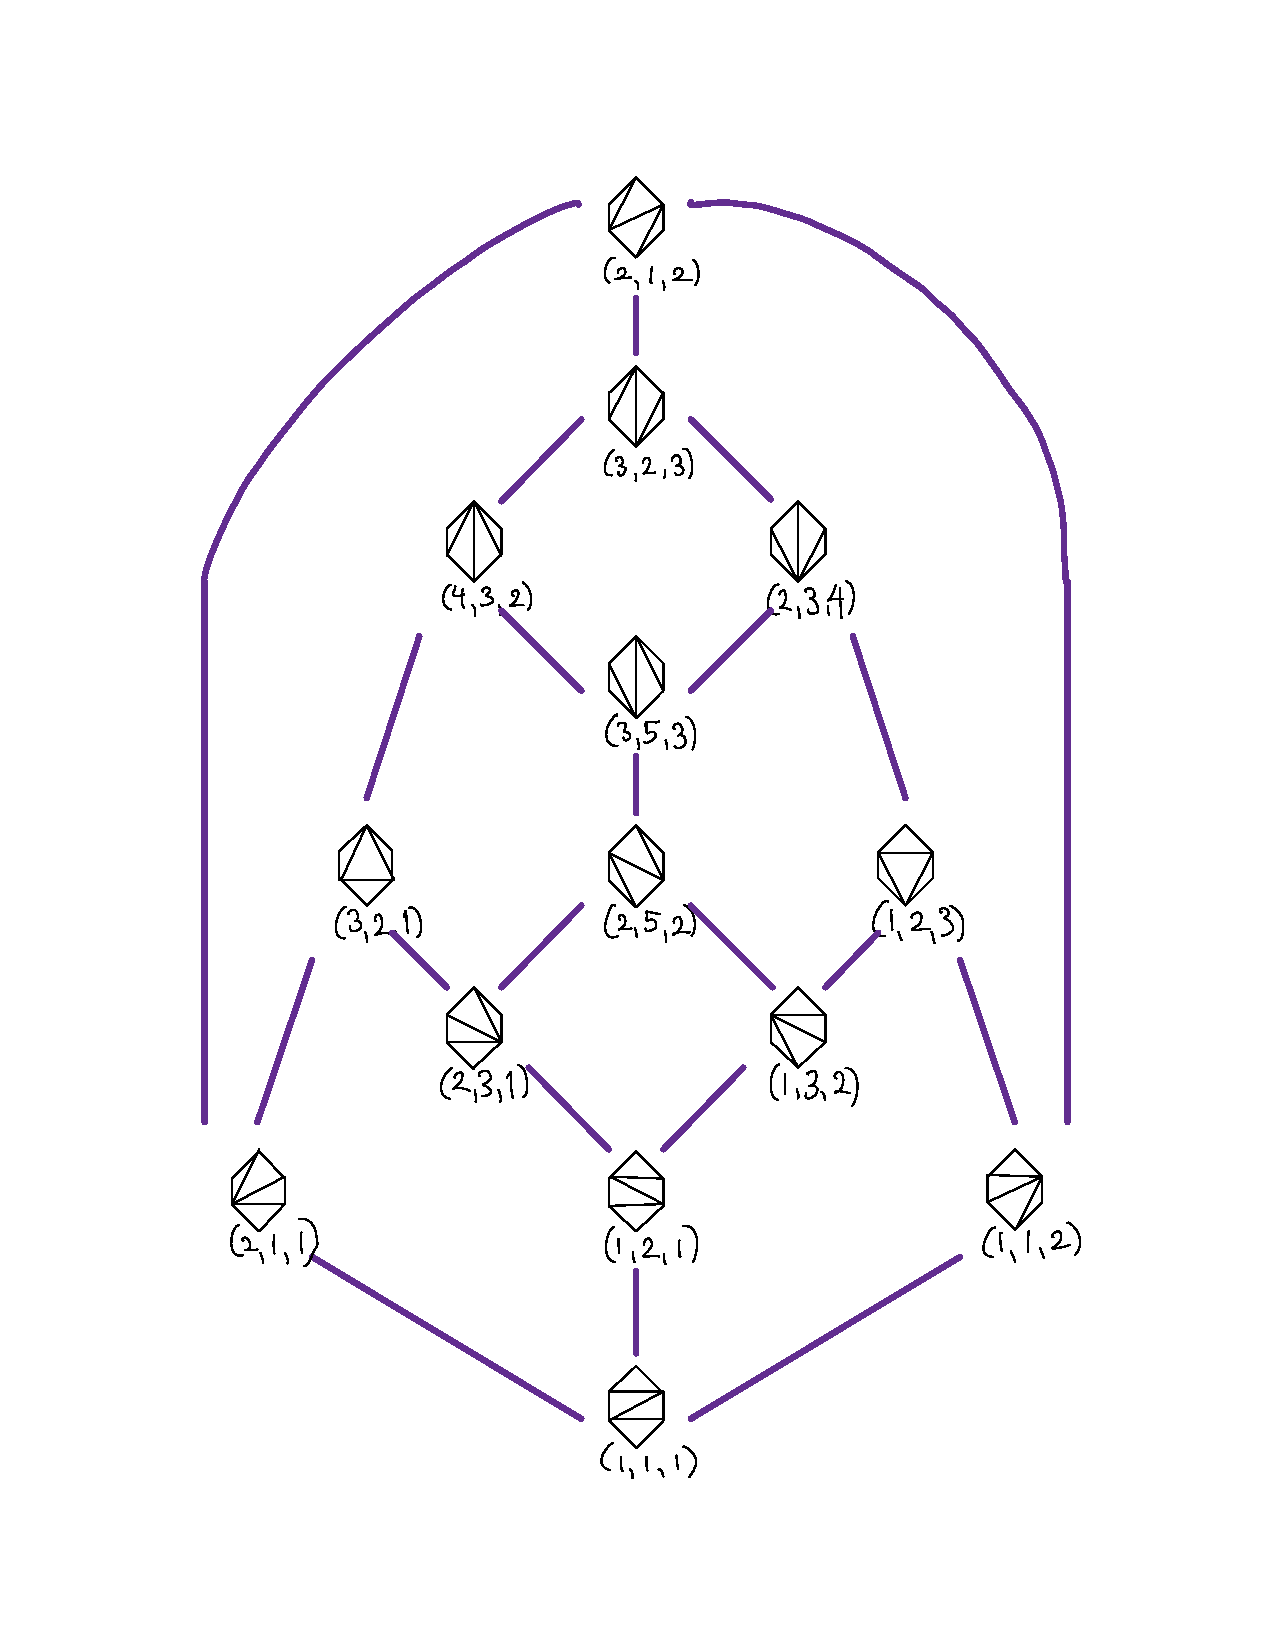
\includegraphics[width=1.20\textwidth]{friezahedron.pdf}
%     \caption{Fourteen frieze vectors relative to $Q=1 \rightarrow 2 \leftarrow 3$}
%\end{figure}     
     \vskip -1.0cm
 \end{center}
    \vskip -1.0cm
      \begin{scriptsize}
      \flushleft
          \vskip -1.7cm
          \hfill
\textcolor{purple}{Frieze vectors relative to $Q=1 \rightarrow 2 \leftarrow 3$}
\end{scriptsize}
\end{column}
\end{columns}
\end{frame}





\begin{frame}
\frametitle{Frieze vectors and unitary friezes}
Up to symmetry, there are exactly $2$ positive friezes of type $\widetilde{\mathbb{A}}_{1,2}$. 
%The two positive integral friezes of type $\widetilde{\mathbb{A}}_{1,2}$, up to symmetry. 
\begin{figure}
\begin{center}
\footnotesize
\def\myxscale{0.53}
\def\myyscale{0.85}

\begin{tikzpicture}[xscale=\myxscale, yscale=\myyscale] % A1,2 preprojective component coming from acyclic seed
\node at (-7.3,-1) {$\dots$};
\draw node at (12.5,-1) {$\dots$};

\def\myshift{0.5}

\foreach \n in {-2,...,5}
{
  \foreach \vertex in
  {0,1,2}
  {
    \path[black] (\n*\myshift-\vertex+2*\n,-\vertex) node (x\vertex\n) {};
  }
  \foreach \source/\target in % each loop produces one copy of 2->1->0
  {2/1,1/0}
  {
    \path[->,>=stealth] (x\source\n) edge[blue] (x\target\n);
  }
  \foreach \source/\target in % each loop produces one (bent) arrow of 2->0
  {2/0}
  {
    \path[->,>=stealth] (x\source\n) edge[blue, bend left=55] (x\target\n);
  }  
}

\foreach \nminusone/\n in % each loop produces (1,n-1) -> (2,n) and (0,n-1)->(2,n)
{%-5/-4,-4/-3,-3/-2,
-2/-1,-1/0,0/1,1/2,2/3,3/4,4/5}
{
  \foreach \s/\t in 
  {1/2,0/2,0/1}
  {
    \path[->,>=stealth] (x\s\nminusone) edge[red] (x\t\n);
  } 
}  

\foreach \vertex/\n/\weight in
  {
0/-2/11,1/-2/26,2/-2/41,
0/-1/2,1/-1/3,2/-1/7,
0/0/1,1/0/1,2/0/1,
0/1/7,1/1/3,2/1/2,
0/2/41,1/2/26,2/2/11,
0/3/\ \ 362,1/3/153,2/3/97,
0/4/\ \ \ 2131,1/4/1351,2/4/571,
0/5/\ \ \ \ \ 18817,1/5/7953,2/5/5042
  }
  {
    \path[black] (\n*\myshift-\vertex+2*\n,-\vertex) node (x\vertex\n) {\weight};
  }
\end{tikzpicture}  
\caption{An $\widetilde{\mathbb{A}}_{1,2}$ frieze obtained by specializing the cluster variables of an acyclic seed to $1$. The two peripheral arcs have  frieze values $2$ and $3$.}\label{fig:A1_2_acyclic} 
\vspace{-1mm}
\begin{tikzpicture}[xscale=\myxscale, yscale=\myyscale] 
% A1,2 preprojective component coming from non-acyclic seed
\node at (-7.3,-1) {$\dots$};
\draw node at (12.5,-1) {$\dots$};

\def\myshift{0.5}

\foreach \n in {-2,...,5}
{
  \foreach \vertex in
  {0,1,2}
  {
    \path[black] (\n*\myshift-\vertex+2*\n,-\vertex) node (x\vertex\n) {};
  }
  \foreach \source/\target in % each loop produces one copy of 2->1->0
  {2/1,1/0}
  {
    \path[->,>=stealth] (x\source\n) edge[blue] (x\target\n);
  }
  \foreach \source/\target in % each loop produces one (bent) arrow of 2->0
  {2/0}
  {
    \path[->,>=stealth] (x\source\n) edge[blue, bend left=55] (x\target\n);
  }  
}

\foreach \nminusone/\n in % each loop produces (1,n-1) -> (2,n) and (0,n-1)->(2,n)
{%-5/-4,-4/-3,-3/-2,
-2/-1,-1/0,0/1,1/2,2/3,3/4,4/5}
{
  \foreach \s/\t in 
  {1/2,0/2,0/1}
  {
    \path[->,>=stealth] (x\s\nminusone) edge[red] (x\t\n);
  } 
}  

\foreach \vertex/\n/\weight in
  {
%0/-5/843,1/-5/610,2/-5/2207,
%0/-4/89,1/-4/322,2/-4/233,
%0/-3/47,1/-3/34,2/-3/123,
0/-2/5,1/-2/18,2/-2/13,
0/-1/3,1/-1/2,2/-1/7,
0/0/1,1/0/2,2/0/1,
0/1/7,1/1/2,2/1/3,
0/2/13,1/2/18,2/2/5,
0/3/\ \ 123,1/3/34,2/3/47,
0/4/\ \ 233,1/4/322,2/4/89,
0/5/\ \ \ \ 2207,1/5/610,2/5/843
  }
  {
    \path[black] (\n*\myshift-\vertex+2*\n,-\vertex) node (x\vertex\n) {\weight};
  }

\end{tikzpicture}  
\caption{An $\widetilde{\mathbb{A}}_{1,2}$ frieze obtained by specializing the cluster variables of a non-acyclic seed to $1$. The two peripheral arcs have frieze values $1$ and $5$.}
\label{fig:A1_2_cyclic}
\end{center}
\end{figure}
%%% END FIGURE %%%%
\end{frame}

%\begin{frame}
%   \includegraphics[width=4.4in]
%   {fig56.pdf} 
%\end{frame}








\end{document}


